% Local INT8 vs cloud LLMs on conversational slices (bedrock_llm_report.json); higher is better
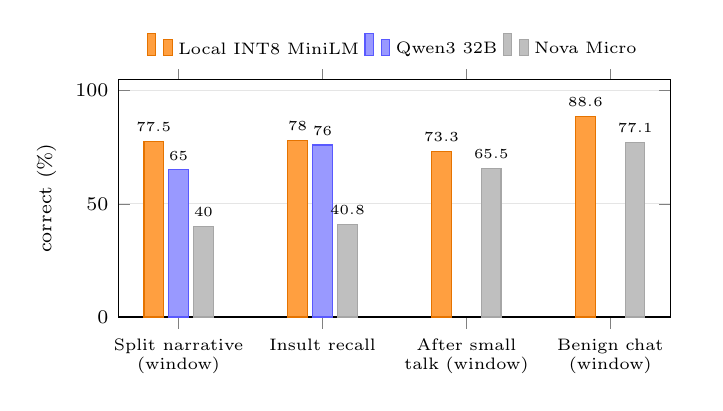
\begin{tikzpicture}
\begin{axis}[ybar, width=8.6cm, height=4.6cm, bar width=7pt, ymajorgrids, grid style={black!10}, ymin=0, ymax=105,
  symbolic x coords={Split narrative (window),Insult recall,After small talk (window),Benign chat (window)},
  xtick={Split narrative (window),Insult recall,After small talk (window),Benign chat (window)},
  x tick label style={font=\fontsize{6.2}{7}\selectfont, text width=1.9cm, align=center},
  tick label style={font=\scriptsize}, label style={font=\scriptsize}, ylabel={correct (\%)}, enlarge x limits=0.14,
  legend style={font=\fontsize{6.5}{7.5}\selectfont, at={(0.5,1.04)}, anchor=south, legend columns=3, draw=none},
  nodes near coords, every node near coord/.append style={font=\fontsize{5.5}{6}\selectfont}]
  \addplot[fill=orange!75, draw=orange!90!black] coordinates {(Split narrative (window),77.5) (Insult recall,78.0) (After small talk (window),73.3) (Benign chat (window),88.6)};
  \addplot[fill=blue!40, draw=blue!65] coordinates {(Split narrative (window),65.0) (Insult recall,76.0)};
  \addplot[fill=gray!50, draw=gray!70] coordinates {(Split narrative (window),40.0) (Insult recall,40.8) (After small talk (window),65.5) (Benign chat (window),77.1)};
  \legend{Local INT8 MiniLM, Qwen3 32B, Nova Micro}
\end{axis}
\end{tikzpicture}
